\setlength{\parskip}{\baselineskip} 
\section{\bnmf}

\begin{frame}
 \frametitle{Table of Contents}
 \vspace{-1em}
\textbf{
\begin{itemize}
 {\color{gray}
     \item {Background}}
     {\color{gray}
         \item {PCP}}
         \begin{itemize}
         {\color{gray}
             \item Method
             \item Simulations
             \item Application}
         \end{itemize}
          {\color{matbluedark}
         \item \textbf{\bnmf}}
         \begin{itemize}
         {\color{gray}
             \item Method
             \item Simulations
             \item Application}
         \end{itemize}
     {\color{gray}
     \item \bnmf \& Child IQ
     \item Conclusion
     }
 \end{itemize}}
\end{frame}

% 	\item[\checkmark] Non-parametric prior on $k$ helps with model selection
% 	\item[\checkmark] Bayesian framework allows uncertainty propagation
%       	\end{itemize}
% }

\frame{
\frametitle{Bayesian non-parametric non-negative matrix factorization (BN$^{2}$MF)}

\centering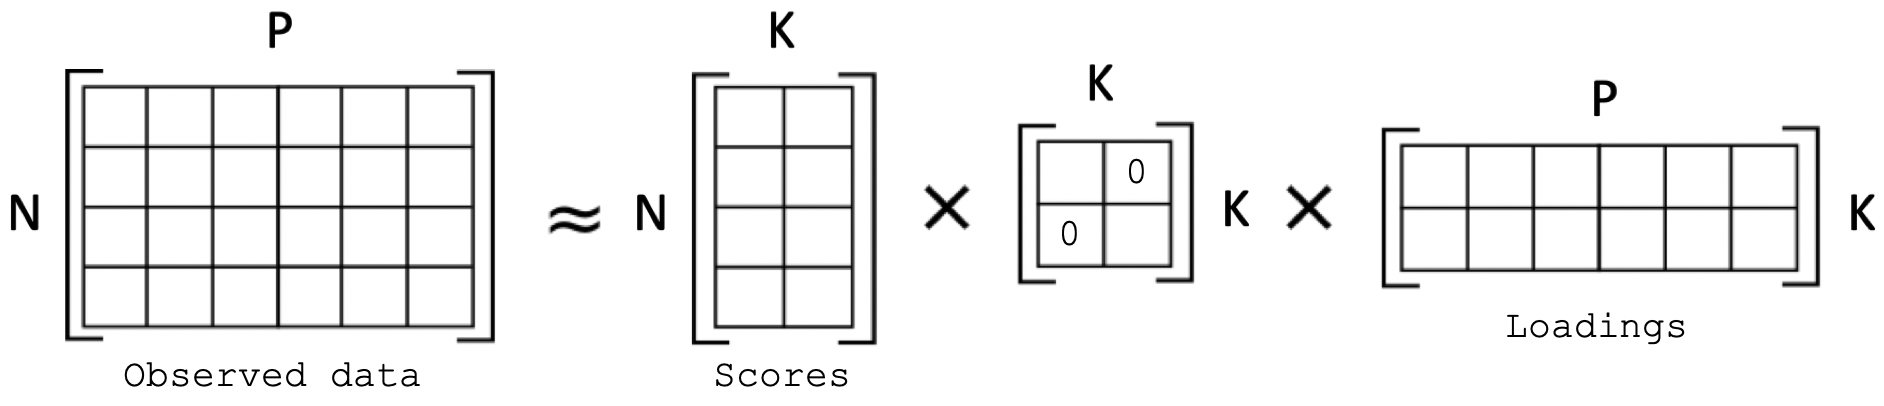
\includegraphics[scale = 0.325]{figures/decomp.png}

\begin{itemize}
\item[$\checkmark$] Non-negative continuous Gamma priors 
\item[$\checkmark$] Sparse non-parametric prior on $k$ estimates pattern number
\item[$\checkmark$] Variational confidence intervals
\begin{itemize}	
\item[\aritem] Bayesian framework allows uncertainty propagation
      	\end{itemize}
\end{itemize}
}

% \frame{
% \frametitle{Non-parametric Bayesian Non-negative Matrix Factorization}
% $$ X_{i j} \sim \operatorname{Poisson}\left(\sum_{k=1}^{K} H_{i k} (a_k) W_{k j}\right)$$
% $$i=1 \ldots n,  j=1 \ldots p,  k = 1 \ldots K$$
% $$ H_{i k} \sim \operatorname{Gamma}(1, 1), 
% \space a_k \sim \operatorname{Gamma}(1 / K, 1), 
% \space W_{k j} \sim \operatorname{Gamma}(1, 1) $$
% \vspace{1ex}
% $$ \underbrace{\Prob{H, \operatorname{diag}(\mathbf{a}), W}}_{\text{Posterior}}
%     \propto \underbrace{\Prob{x \mid H, \operatorname{diag}(\mathbf{a}), W}}_{\text{Likelihood}}
%     \times \underbrace{\Prob{H, \operatorname{diag}(\mathbf{a}), W}}_{\text{Prior}} $$
% }